
\section{Experiment}
\label{ch:experiment}

\epigraph{That men do not learn very much from the lessons of history is the most important of all the lessons that history has to teach.}{Aldous Huxley}

\subsection{User Study Process}
Let users use our recommendation system, record their feedback and answers to the questionnaires, and analyze data to evaluate the performance and interpretability of our recommendation system.
\par After reading the explanations about the user study, users will input some personal data (user id, gender, age and occupation) and then answer some background questions. For building user Pprtraits, system will give user a series of movie posters and names. user can click to select the movies he likes from 6 options. Click the ?REFRESH? button to load the new 6 options and repeat this selection process until the user has selected a total of 10 movies. After that, the system will give user a series of recommendation movies and the explanations why these are recommended to the user. The user can click to select the movies he likes and give a score for the explanations. Repeat this recommendation step three times. Finally, the user will be required to answer some feedback questions.

\subsection{likert Scale}
The statistics of the questionnaire about system evaluation by using likert scale are shown in figure \ref{figure:1}.

\begin{figure}[h]
\caption{Feedback question about system evaluation}
\label{figure:1}
\centering
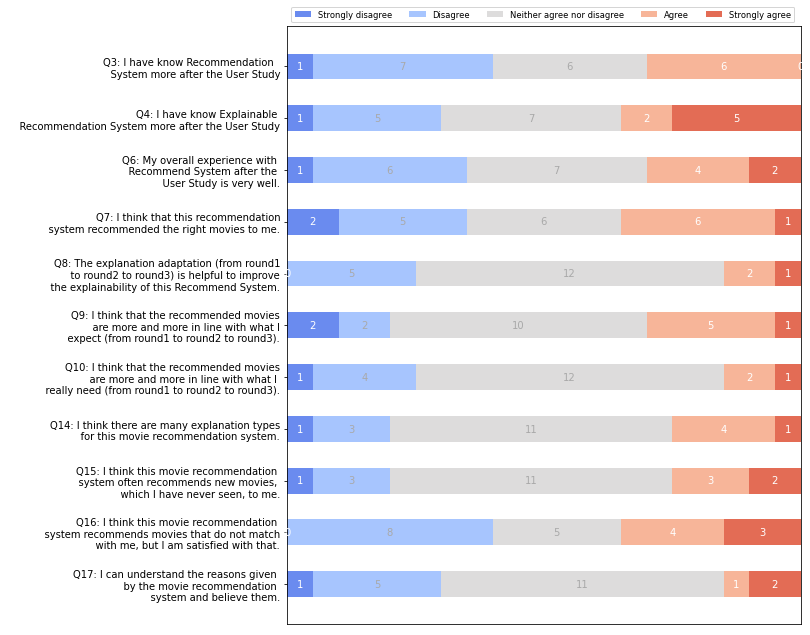
\includegraphics[width=1\textwidth]{feedback_question3}
\end{figure}

Figure \ref{figure:2} presents the results obtained from the preliminary analysis of points for 3 round recommendations from 20 users. We can see that the third round reported more high-points than the other two rounds. This shows that in our user study, the average score of users improved through three rounds of explanation adaptation.

\begin{figure}[h]
\caption{Feedback question about 3 round recommendations}
\label{figure:2}
\centering
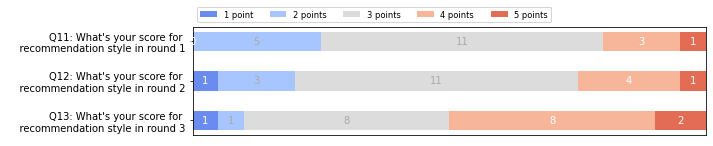
\includegraphics[width=1\textwidth]{feedback_question2}
\end{figure}



\subsection{User Study Metric}
Correspondingly, the division of questions for evaluating the recommendation system is shown in the table \ref{table:1}.

\begin{table}[h!]
\renewcommand\arraystretch{1.5}
\centering
\begin{tabular}{p{100pt}p{60pt}p{200pt}}\toprule
 \hline
 System Evaluation & Question & Result \\ [0.5ex] 
 \hline
  Satisfaction & Q8 & More than half of users choose a neutral attitude (12 in 20)  \\
   \cdashline{1-3}[0.8pt/2pt]
    & Q7 & 7 users agree that the system recommend the right movies.\\
  Accuracy  & Q9 & 6 users agree that the system has recommended what they expect. \\
    & Q10 & 3 users agree that the system has recommended what they really need. \\
    \cdashline{1-3}[0.8pt/2pt]
  Diversity & Q14 & 5 users agree \\
  Novelty & Q15 & 5 users agree \\
  Surprise & Q16 & 7 users agree \\
  Trust & Q17 & 3 users agree \\
  [1ex] 
 \hline
\end{tabular}
\caption{Questions for system evaluation}
\label{table:1}
\end{table}

\paragraph{Confidence:}
\paragraph{Transparency:}
\paragraph{Satisfaction:}
\paragraph{Accuracy:}
Comparing the three questions about accuracy ( Q7, Q9, Q10), we can find a very interesting phenomenon. Some users said that the recommendation system recommended the right movies to them, but they thought that the recommendation system did not recommend the movies they really expected and needed.
\par As Abraham argues in \cite{maslow1943theory} about Maslow's hierarchy of needs, from low to high, human needs are divided into physiological needs, safety needs, social needs, esteem and self-actualization needs.
\par Most recommendation systems, including our recommendation system, often recommend things that users may be interested in based on some data and records. This is certainly the right recommendation, but sometimes it may not be what users really expect and demand. The recommended things only satisfy the user's physiological needs, safety needs, and social needs. And higher-level esteem and self-actualization needs may become one of the possible development directions of future recommendation systems research area.
	
\subsection{Result analysis}

\cleardoublepage